

% File: formatting-instruction.tex
\documentclass[letterpaper]{article}
\usepackage{aaai}



\usepackage{times}
\usepackage{helvet}
\usepackage{courier}


\newcommand{\solver}[1]{{\sc #1}}
\newcommand{\system}[1]{\solver{#1}}
\newcommand{\problem}[1]{{\rm #1}}
\newcommand{\pcogx}{\solver{PCogX}}

\newcommand{\assumptiveS}[1]{\actions^{\circ}(p_{#1};T_{#1})}
\newcommand{\assumptiveDT}[1]{\actions^{\bullet}(p_{#1};T_{#1})}


\newcommand{\actNam}[1]{\texttt{#1}}
\newcommand{\pp}[1]{\actNam{#1}}

\newcommand{\Expect}{\makebox[1em]{$\mathbin{\mbox{\sf E}}$}}

\newtheorem{definition}{Definition}
\newtheorem{proposition}{Proposition}
\newtheorem{lemma}{Lemma}
\newtheorem{theorem}{Theorem}
\newtheorem{property}{Property}
\newtheorem{corollary}{Corollary}

\newcommand{\laostar}{\textsc{lao$^*$}}
\newcommand{\fastdownward}{\textsc{FastDownward}}


\newcommand{\obsDist}{\ensuremath{\mathit{v}}}

\newcommand{\states}{\ensuremath{\mathcal{S}}}
\newcommand{\state}{\ensuremath{s}}
\newcommand{\observ}{\ensuremath{o}}
\newcommand{\observation}{\ensuremath{\observ}}
%% \newcommand{\percept}{\ensuremath{\widetilde{\observ}}}
\newcommand{\reward}{\ensuremath{{\sf R}}}
\newcommand{\transProb}{\ensuremath{{\sf Pr}}}
%% \newcommand{\States}{\ensuremath{\mathbb{S}}}
%% \newcommand{\TransProb}{\ensuremath{\textbf{Pr}}}
%% \newcommand{\Reward}{\ensuremath{\reward}}
%% \newcommand{\Actions}{\ensuremath{\mathbb{A}}}
%% \newcommand{\Observ}{\ensuremath{\mathbb{O}}}
\newcommand{\observations}{\ensuremath{O}}
\newcommand{\policy}{\ensuremath{\pi}}
\newcommand{\actions}{\ensuremath{\mathcal{A}}}
\newcommand{\action}{\ensuremath{a}}

%% \newcommand{\object}{\ensuremath{o}}
%% \newcommand{\objects}{\ensuremath{\mathcal{O}}}

\newcommand{\bstate}{\ensuremath{b}}

\newcommand{\Omit}[1]{}

\newcommand{\props}{\ensuremath{{\cal P}}}
\newcommand{\prop}{\ensuremath{p}}
\newcommand{\propositions}{\props}
\newcommand{\percepts}{\ensuremath{\Pi}}
\newcommand{\percept}{\ensuremath{\pi}}

\newcommand{\stochActions}{\ensuremath{\actions}}
\newcommand{\detActions}{\ensuremath{\actions^d}}
\newcommand{\stochAction}{\ensuremath{\action}}
\newcommand{\detAction}{\ensuremath{\action^d}}
\newcommand{\stochAct}{\stochAction}
\newcommand{\detAct}{\detAction}

\newcommand{\stochSenses}{\ensuremath{K}}
\newcommand{\detSenses}{\ensuremath{K^d}}
\newcommand{\stochSense}{\ensuremath{\kappa}}
\newcommand{\detSense}{\ensuremath{\kappa^d}}


\newcommand{\poss}{\ensuremath{\pp{poss}}}
\newcommand{\add}{\ensuremath{\pp{ add}}}
\newcommand{\delete}{\ensuremath{\pp{delete}}}



\newcommand{\nodes}{\ensuremath{\mathcal{N}}}
\newcommand{\selections}{\ensuremath{\Psi}}
\newcommand{\transitions}{\ensuremath{\Eta}}
\newcommand{\node}{\ensuremath{n}}
\newcommand{\selection}{\ensuremath{\psi}}
\newcommand{\transition}{\ensuremath{\eta}}


\def\oom{$^{\tt +}$}
\def\zom{$^*$}
\def\bump{\hspace{1cm}}
\newenvironment{tabtt}{\begin{tt}\begin{tabbing}}{\end{tabbing}\end{tt}}


\def\oom{$^{\tt +}$}
\def\zom{$^*$}
\def\bump{\hspace{1cm}}
\def\req#1{$^{\tt #1}$}
\def\noteme#1{}%{[[#1]]}
\def\notecoauth#1{\ }
\def\notereader#1{[[#1]]}
\def\meta{$\uparrow\uparrow$}
\def\la{\langle}
\def\ra{\rangle}
%

\nocopyright

\pdfinfo{
/Title (Switching in Continual Planning for Practical Robot Control)
/Subject (Proceedings of the 21st International Conference on Automated Planning and Scheduling)
/Author (NA)}
% The file aaai.sty is the style file for AAAI Press 
% proceedings, working notes, and technical reports.
%
%\title{Switching in Continual Planning for Practical Robot Control}
\title{A Switching Planner for Combined Task and Observation Planning}
%\title{A Continual Planner that Switches Between Sequential and
%  Decision-Theoretic Planning} 
\author{NA}
\setcounter{secnumdepth}{0}


\begin{document} 
\maketitle

\begin{abstract}

Realistic robot planning problems in uncertain environments often
require achieving tasks while also finding out about the
world. Because the world state cannot be observed directly, these
problems are naturally represented as partially observable Markov
decision problems (POMDPs). However, these are typically intractable
for realistic problems.

We present a \emph{switching planner} that employs fast sequential
planning to decide on the overall strategy, and uses a
decision-theoretic planner to solve the subproblems where partial
observability will significantly impact the quality of the plan. We
demonstrate the approach in a realistic robot exploration domain.

\end{abstract}

\section{Moritz's Initial Outline}

\subsection{Switching Planner Outline}

Outline the high level approach here:
\begin{itemize}
\item Problem input (factored initial state, DTPDDL observations)
\item Determinisation
\item Problem generation for DT
\item Belief revision
\end{itemize}

\subsection{Determinisation}

\begin{itemize}
\item Generation of deterministic sensing models
\item Determinisation of the initial state
\item Compiling reward model into (soft-)goal model
\item Cost function in FD (maybe this could mentioned in the outline?)
\end{itemize}

\subsection{Subtask Generation}
\begin{itemize}
\item Goal generation from CP trace
\item Disconfirm actions
\item State pruning according to CP trace
\end{itemize}

\subsection{Belief revision}
Not sure if this needs its own section
\begin{itemize}
\item Convert inital state into bayesian network
\item Belief updates with observation nodes
\item Create new network for next planning runs
\end{itemize}

\section{Introduction}





Recently there have been a number of integrated robotic systems which
incorporate a high-level {\em continual planning} and execution
monitoring
subsystem~\cite{wyattetal2010tamd,talamadupula:2010,Kraft2008}.
%%
For the purpose of planning, sensing is modelled {\em
deterministically}, and beliefs about the underlying state are
modelled {\em qualitatively}.
%%
Both~\citeauthor{talamadupula:2010} and
~\citeauthor{wyattetal2010tamd} identify
\emph{continual planning} with {\em probabilistic}
models as an important challenge for future research.
%%
Motivating that sentiment, planning according to an accurate
stochastic model of noisy sensing and state should yield more
efficient and robust deliberations.
%%
In the first place, that means moving from deterministic to
probabilistic models of noisy sensing, and from qualitative to
quantitative models of state uncertainty. The key challenge then, is
to develop a {\em base planner} that exhibits similar speed and
scalability to base planners employed in existing robotic systems
---e.g.,~\citeauthor{wyattetal2010tamd} use a {\em classical}
procedure--- which is also able to synthesise relatively efficient
deliberations according to detailed probabilistic models of the
environment.


This paper describes a planning approach we have developed to address
the challenge just outlined. The approach is implemented on a mobile
robotic platform that continuously deliberates in a stochastic dynamic
environment in order to achieve goals set by the user, and acquire
knowledge about its surroundings.


This domain features partial observability, particularly
because the state is not perfectly known, and state information is
gained by the robot through the use of noisy sensing
actions. 
%Using a propositionally factored state representation, for
For
interesting sized tasks the corresponding POMDP model is too large for a
POMDP solver to be applied directly. Inspired by the replanning
approaches used successfully for MDP
planning~\cite{yoon:etal:2007,yoon:etal:2008}, we propose a continual
planning approach that uses a classical planning system to compute a
reasonably valuable trace in the model, and then uses a
decision-theoretic planner on small subproblems where reasoning about
observations might be useful. We refer to the complete system as a
{\em switching continual planner}. The approach is not optimal,
particularly as it relies on the results of satisficing sequential planning
directly. It does nevertheless perform better than a purely sequential
replanner, and is fast enough to be used for real-time decision-making
on a mobile robot.





Our system is domain independent, taking domain and problem
descriptions in a first-order declarative language we have developed,
called the decision-theoretic planning domain definition language
(DTPDDL). In this paper, we restrict our attention to deterministic
action goal-oriented POMDPs\foonote{We note that POMDPs with
stochastic actions can be compiled into equivalent
deterministic-action POMDPs, where all the original action uncertainty
is expressed in the starting-state
distribution~\cite{ng:Jordan:2000}.} -- I.e., where a finite horizon
optimal contingent plan exists.  
%%
From these descriptions of POMDPs, we
automatically construct a deterministic model for the sequential
planner. That model includes actions which correspond to making
assumptions about the values of imperfectly known state
variables. Assumptions scheduled by the sequential system are used to
propose a pragmatic abstract belief-state space to the
decision-theoretic system, and to modify the reward function, so that
system might pursue sensing related to those assumptions.


The switching planner provides important advantages in our
mobile robot domain. First, the significant source of uncertainty in the
domain is the unreliability of observations and this approach is
particularly suited to problems that combine a deterministic task
planning problem with observations because the decision-theoretic planner
is only invoked to deal with state uncertainty.
%determine a characteristic of the underlying state. 
Secondly, replanning makes the system robust to
changing objectives and discoveries about the world,
both of which feature in our domain.



The remainder of the paper proceeds as follows. We begin by describing
related work. Next we describe our DTPDDL language with example
declarations from a mobile robot exploration task. Then we describe
the switching planner, how sequential planning proceeds in our problem
models, and how this then provides the input for the
decision-theoretic planner. Finally we provide an evaluation of the
system on the example robot domain, and then provide some concluding
remarks and future directions.





%% BEGIN SCRAPPY


%% The initial abstract process, let's suppose, has two states. The state
%% where everything assumed is true, and the null state. This has a KL
%% divergence from the :init term, because we can suppose it uniformly
%% chooses one concrete state, given the abstract :init states.

%% As you add propositions to the abstract :init term, then the KL
%% divergence decreases. 


%% END SCRAPPY

%%
%% The underlying planning procedures are {\em classical}, i.e.,
%% sequential, planning system.



%% Planning for agents acting in partially observable environments with
%% stochastic actions is extremely computationally
%% expensive~\cite{mdp-complexity}. Even relatively small partially
%% observable Markov decision problems (POMDPs), represented by tens of
%% propositional variables, have state spaces far larger than existing
%% optimal or close to optimal planners can handle. For the easier
%% problem of planning in completely observable stochastic domains, an
%% alternative has been to use classical sequential planners and
%% replan when actions have unplanned-for outcomes~\cite{yoon:etal:2007}.
%% Execution monitoring tracks properties of the state that determine
%% whether further planning is required. For partially observable
%% domains, only probabilistic information about such properties will, in
%% general, be available.



%% However, these approaches rely
%% crucially on being able to determine properties of the current state
%% in order to decide to replan. For partially observable domains, only
%% probabilistic information about these properties will in general be
%% available.



%% Switching gives us some important advantages in our robotic
%% domain. First, the significant source of uncertainty in the domain is
%% the unreliability of observations, and this approach is particularly
%% suited to problems that combine a deterministic task planning problem
%% with observations as the decision-theoretic planner is often invoked
%% to determine a characteristic of the underlying state. Secondly,
%% replanning makes our system robust to changing objectives and the
%% discovery of new facts about the world.


%% As an illustration, consider a robot searching for a box that it knows
%% is often found in offices. The sequential planner might produce a plan
%% that assumes that {\sc Room a} is an office, that the box is in {\sc
%% Room a}, and that the box is in location 1 in {\sc Room a}. Given
%% these assumptions, the plan might be to go to {\sc Room a}, go to
%% location 1 and search for the box. When the plan gets executed and the
%% search begins the decision-theoretic planner is called since searching
%% involves making observations. The decision-theoretic planner might
%% retract the last assumption but leave the others, and build a plan to
%% search the whole of {\sc Room a} for the box. If this plan fails to
%% find the box, it will disprove the assumption that the box is in {\sc
%% Room a}, which will then lead to replanning by the sequential planner
%% based on the newly discovered knowledge.


%To accompany
%that language we have implemented an information-state
%\laostar\ procedure for solving problems expressed in DTPDDL. 

%%

%Have a good understanding of the contents and function of rooms, as
%well as the linguistic referrents to rooms, widgets, and their visual
%qualities.

%Having confidence in its beliefs about the linguistic terms for
%spaces, and the function of those spaces.



%sometimes difficult to predict, with exogenous events, such as the
%changing of the objective, 





%the speed and scalability of software for sequential planning in
%deterministic




%% We developed a first-order declarative language, called DTPDDL, for
%% describing domains of planning problems that correspond to POMDPs.  To
%% accompany that language we have implemented an information-state
%% \laostar\ procedure for solving problems expressed in DTPDDL. 

%% We have extended MAPSIM to parse and simulate DTPDDL problems, and
%% modified \fastdownward\ so that it can find useful sequential executions
%% given DTPDDL models of the problem at hand.




%%  called DTPDDL, along
%% the lines of PDDL for the partially observable case, an \laostar\
%% solution procedure, a determinisation of the DTPDDL problem in MAPL,
%% and modify the \fastdownward\ system to find high quality sequential plans
%% .

%% We model the environment as a partially observable Markov decision
%% process. Although planning in that model is undecidable in
%% general~\cite{}, an optimal finite-horizon plan corresponds to a
%% contingent plan, that is a function mapping action-observation
%% histories to actions.

%% our continual planner is reactive, replanning whenever the underlying
%% domain and problem models change. For example, replanning occurs if
%% the motivational component alters the objectives, and if an assumed
%% outcome of a sensing action is not realised.

%% brittle sensing model, 

%% the evaluation of a fluent at a state is either known. Moreover, there
%% is a sensing process that run-time variables  after-which 

%% For $\prop \in \state$ we say proposition $\prop$ characterises state
%% $\state$. There is always a unique starting state $\state_0$. The goal
%% $\goal$ is a set of propositions, and we say that state $\state$ is a
%% goal state iff $\goal \subseteq \state$.

%%  To keep this exposition
%% simple, for any two distinct actions $\stochAction_i \neq
%% \stochAction_j$, if outcome $\detAct$ is a possibility for
%% $\stochAction_i$ then it cannot also be a possibility for
%% $\stochAction_j$ -- i.e., if $\detAct \in
%% \detActions(\stochAction_i)$ then $\detAct \not\in
%% \detActions(\stochAction_j)$.


%% The solution to a probabilistic planning problem is a contingency
%% plan. This consists of an assignment of actions to states at each
%% discrete timestep up to the planning horizon $n$. The optimal
%% contingency plan is one which prescribes actions to states that
%% maximise the probability that the goal is achieved within $n$ steps
%% from the starting state $\state_0$. For the purposes of this paper
%% we say a plan fails, i.e. achieves the goal with probability $0$, in
%% situations where it does not prescribe an action. Computing the
%% optimal plan for a problem is computationally intractable, and an
%% important direction for research in the field is to develop
%% heuristic mechanisms for generating small linear plans
%% quickly~\cite{littman:etal:98}

%%  which can operate
%% with the original representation of the domain.


%% The sequential planner we use is based
%% on \fastdownward~\cite{fast-downward}. We add the capability to replan
%% ~\cite{brenner:nebel:jaamas09}, and also allow agent
%% knowledge to be represented explicitly, so we can write actions that
%% gain the agent knowledge. LEASE CITE MICHAEL's WORK AS THE BASIS FOR
%% THIS. For the decision-theoretic planner we have implemented our own
%% forward search in the belief-state space.


\section{Propositional Decision-Theoretic Planning}

%% {\em runtime variables}
%% {\em decision variables}
%% {\em uninitialised variables}
%% {\em omitted variables}

We describe the partially observable propositional probabilistic
planning problem, with costs and rewards. We model a process
state $\state$ as the set of propositions that are true of the
state. Notationally, we have $\state \subseteq
\props$. The underlying process
dynamics are modelled in terms of a finite set of {\em probabilistic
STRIPS operators}~\cite{boutilier:1996} $\stochActions$ over
state-characterising propositions $\propositions$.
%%
Notationally, we say an action $\stochAction \in \stochActions$ is
applicable if its precondition $\poss(\stochAction)$, a set of
propositions, are satisfied in the current state -- i.e., $\poss(\stochAction) \subseteq
\state$. We denote $\mu_{\stochAction}(\detAction_i)$ the probability that
nature chooses a deterministic STRIPS effect $\detAct_i$, and for
all \stochAction\ we require
$\sum_{\detAction_i \in \detActions(\stochAction)}
\mu_{\stochAction}(\detAction_i) = 1$.

%% We model a process state $\state$ as the set of propositions that are
%% true of the state. Notationally, we have $\state \subseteq
%% \props$. State change is induced by application of actions. A
%% stochastic action $\stochAction \in \stochActions$ is applicable if
%% its precondition $\poss(\stochAction)$, a set of propositions, are
%% satisfied in the current state. We write $\stochActions(\state)$ for set of actions
%% applicable at state $\state$.  If action $\stochAction \in
%% \stochActions(\state)$ is applied at \state, nature chooses one
%% element amongst a small set of deterministic outcomes
%% $\detActions(\stochAction) \equiv \{\detAction_1, \ldots, \detAction_k
%% \}$. We denote $\mu_{\stochAction}(\detAction_i)$ the probability that
%% nature takes outcome $\detAct_i$, and for all \stochAction\ we require
%% $\sum_{\detAction_i \in \detActions(\stochAction)}
%% \mu_{\stochAction}(\detAction_i) = 1$. The chosen outcome has an
%% effect on the state given in terms of two lists of propositions. The
%% add-list $\add(\detAction)$ and delete-list
%% $\delete(\detAction)$.\footnote{If a proposition is in the add-list of
%% $\detAction$, then it cannot be in the delete-list and vice versa.}
%% If outcome $\detAction$ with $\add(\detAction) := [\prop_1,
%% ..,\prop_n]$ and $\delete(\detAction) := [\prop_{n+1},
%% ..,\prop_m]$ is chosen by nature when \stochAction\ is
%% applied at state $\state$, then the resultant state is $ ( \state \cup
%% \add(\detAction) ) \backslash \delete(\detAction)$ -- i.e.,
%% propositions from $\add(\detAction)$ are added to $\state$, and those
%% from $\delete(\detAction)$ are removed from $\state$.

%% \citeauthor{rintanen:01}~(\citeyear{rintanen:01})

We are concerned with problems that feature partial
observability. Although we could invoke {\em extended probabilistic
STRIPS operators}~\cite{rintanen:01} to model actions and observations
propositionally, we find it convenient for our presentation to clearly
separate sensing and action. Therefore, we suppose a POMDP has a
perceptual model given in terms of a finite set of stochastic {\em
senses} $\stochSenses$, deterministic sensing outcomes $\detSenses$,
and perceptual propositions $\percepts$, called {\em percepts}. In
detail, we take an observation $\observ$ to be a set of percepts
$\observ \subseteq \percepts$, and denote \observations\ the set of
reachable observations. The underlying state of the process cannot be
observed directly, rather, senses $\stochSense \in \stochSenses$
effect an observation $\observ \in
\observations$ that informs what should be believed about the state a
process is in. In detail, if $\action$ is applied effecting a
transition to a successor state $\state'$, then an observation occurs
according to the active senses $\stochSenses(\stochAction, \state')
\subseteq \stochSenses$. A sense $\stochSense$ is active, written
$\stochSense \in \stochSenses(\stochAction, \state')$, if the senses'
action-precondition, $\poss_\stochActions(\stochSense)$, is equal to
$\stochAction$, and the state-precondition $\poss_\states(\stochSense)
\subseteq \propositions$ is satisfied by the state $\state'$; In the
usual sense that $\poss_\states(\stochSense) \subseteq \state'$.
%%
When a sense is active, nature must choose exactly one outcome amongst
a small set of deterministic choices $\detSenses(\stochSense)
\equiv \{\detSense_1, \ldots, \detSense_k \}$, so that for each
$i$ we have $\detSense_i \subseteq \percepts$. The probability of
the $i^{th}$ element being chosen is given by
$\psi_{\stochSense}(\detSense_i)$, where $\sum_{\detSense_i \in
\detSenses(\stochSense)} \psi_{\stochSense}(\detSense_i) =
1$. The observation received by the agent corresponds to the union of
perceptual propositions from chosen elements of active
senses.

A POMDP has a starting configuration that corresponds to a Bayesian
belief-state. Intuitively, this is the robot's subjective belief about
its environment. Formally, a belief-state $\bstate$ is a probability
distribution over process states. We write $\bstate(\state)$ to denote
the probability that the process is in $\state$ according to
$\bstate$, and $\bstate_0$ when discussing the starting
configuration. 

Finally, we make a number of fairly standard assumptions. First, that
action execution and sensing occurs instantaneously, and that only one
action can be applied at a plan-step. Second, it can arise that in
some propositional states an action is applicable, and in others it is
not. Moreover, a belief-state can assign non-zero probability to
states where that applicability holds, and states where it does
not. We differ
from~\citeauthor{younes:littman:04}~(\citeyear{younes:littman:04}),
because we forbid the execution of actions that are not applicable in
any state of the current belief.  Also,
unlike~\citeauthor{hoffmann:brafman:2006}~(\citeyear{hoffmann:brafman:2006}),
we do incorporate a PPDDL-like default semantics, treating an action
\stochAction\ executed at $\state_i$ as if it has no effect at
states $\state$ if $\poss(\stochAction) \not\subseteq
\state$.


\subsection{Costs, Rewards, and Belief Revision}

Until now we have discussed the POMDP in terms of propositions and
percepts. In order to address belief revision and utility it is
convenient to consider the underlying decision process in a flat
format. This is given by the tuple
$\langle \states, \bstate_0, \actions, \transProb, \reward,
\observations, \obsDist \rangle$. Here $\bstate_0$ is the initial
belief-state, \states\ is the finite set of reachable propositional
states, \actions\ is the finite set of actions, and \observations\ is
the finite set of reachable observations (i.e., perceptual states).
Where $\state, \state' \in \states$, $a \in \actions$, from $\mu$ we
have a state transition function $\transProb(\state, \action,
\state')$ giving the probability of a transition from state $s$ to
$s'$ if $a$ is applied. For any $\state$ and $\action$ we have
$\sum_{\state' \in \states} \transProb(\state, \action, \state') = 1$.
%%
Function $\reward:\states \times \actions \to \Re$ is a bounded real
valued reward function. Therefore a finite positive constant $c$
exists so that for all $\state \in \states$ and $\action \in
\actions$, $|\reward(\state, \action)| < c$. We model costs as
negative rewards.
%%
From $\psi$ we have that for each $\state \in \states$ and action
$\action \in \actions$, an observation $\observ \in \observations$ is
generated independently according to a probability distribution
$\obsDist(\state, \action)$. We denote $\obsDist_\observ(\state,
\action)$ the probability of getting observation $\observ$ in state
$\state$. For $\state$ and $\action$ we have $\sum_{\observ \in
\observations} \obsDist_\observ(\state, \action) = 1$.

Successive state estimation is available by application of Bayes'
rule.  Taking the current belief $\bstate$ as the {\em prior}, and
supposing action $\action$ is executed with perceptive outcome
$\observ$, then the probability that we are in $\state$ in the
successive belief-state $\bstate'$ is given by:

\begin{equation}\label{eq:revision}
\bstate'(\state) = \frac{\obsDist_\observ(\state, \action)
  \sum_{\state'\in \states} \transProb(\state', \action, \state) \bstate(\state') }{\pp{Pr}(\observ | \action, \bstate)}
\end{equation}

\noindent where $\pp{Pr}(\observ | \action, \bstate)$ is the
normalising factor, that is, the probability of getting observation
$\observ$ given we execute $\action$ in $\bstate$.

\subsection{Plan Evaluation}

An optimal solution to a finite-horizon POMDP is a contingent plan,
and can be expressed as a mapping from observation histories to
actions. Although suboptimal in general, useful plans can also take a
classical sequential format. This is the case in {\em conformant}
planning, where the objective is to find a sequence of actions that
achieves a goal ---i.e., reaches a state that satisfies a given
Boolean condition--- with probability $1$.  Generally, whatever the
structure of a plan, its value corresponds to the expected cumulative
reward:

%% More generally, a useful
%% formalism for representing solutions to POMDPs is the finite-state
%% controller (FSC). This is a three-tuple $\langle \nodes, \selection,
%% \transition \rangle$ where: $\node \in \nodes$ is a set of controller
%% states, $\selection_\node(\action) = P(\action | \node)$ gives the
%% probability that the controller prescribes \action\ when in state
%% \node, and $\transition_\node(\action, \observation, \node') =
%% P(\node'|\node, \action, \observation)$ gives the probability the
%% controller transitions to state $\node'$, supposing we execute
%% \action\ in state \node\ receiving observation \observation. When
%% acting for finite $N$ steps from controller state $n$, the value of a
%% controller corresponds to the expected cumulative reward:

\begin{equation}\label{eq:expectedvalue}
V_{\pp{PLAN}}(\bstate) = \Expect \bigg{[} 
\sum_{t=0}^{N-1}  \reward(\bstate_t, \pp{PLAN}_t) \mid \pp{PLAN}, \bstate_0 = \bstate \bigg{]}
\end{equation}

\noindent Where $b_t$ is the belief-state at step $t$, $\pp{PLAN}_t$ is
the action prescribed at step $t$, and

\[\reward(\bstate, \action) = \sum_{\state \in \states}
\bstate(\state)\reward(\state, \action).\] 

%% \noindent Finally, it is
%% useful to note that there is a corresponding deterministic FSCs for
%% both sequential (e.g., conformant) and contingent plan formats.



\section{Decision-Theoretic PDDL}



We give an overview of the declarative first-order language DTPDDL, an
extension of PPDDL that can express probabilistic models of the
sensing consequences of acting, to quantitatively capture
unreliability in perception. There are straightforward compilations
from problems expressed in DTPDDL to flat (and factored)
representations of the underlying decision process. Although similar
to Bryce's POND input language, DTPDDL distinguishes itself by
explicitly treating state and perceptual symbols separately, and by
providing distinct declarations for operators (i.e, state model) and
senses (i.e., observation model). In this last respect, DTPDDL admits
more compact domain descriptions where sensing effects are common
across multiple operators. In detail, DTPDDL has perceptual analogues of
fluent and predicate symbols. For example, a simple {\em object search}
domain would have:

\vspace{-1ex}
\small
\begin{tabtt}
(\=:functions  ;; state fluents\\
  \> (is-in ?v - visual-object) - location )\\
(:perceptual-functions  ;; perceptual fluents\\
  \> (o-is-in ?v - visual-object) - location )
\end{tabtt}
\normalsize
\vspace{-1ex}

\noindent Where the first fluent symbol models the actual location of
objects, and the second the instantaneous sensing of objects
following application of an action with sensing consequences.
%%
To model sensing capabilities, we have operator-like ``sense''
declarations, with preconditions expressed using state and action
symbols, and uniformly positive effects over perceptual symbols. For
example, where {\em look-for-object} is the operator that applies an
object detection algorithm at a specific place, an {\em
object search} task will have:

\vspace{-1ex}
\small
\begin{tabtt}
(\= :sense vision  :parameters \+ \\
  (?r -robot ?v -visual-object ?l -location) \\
 :execution  (look-for-object ?r ?v ?l) \\
 :precondition (and (= (is-in ?r) ?l) ) \\
 :\=effect (and \+\\
    (\= when (= (is-in ?v) ?l)\\
    \>(probabilistic .8 (= (o-is-in ?v) ?l))) \\
   (when (not (= (is-in ?v) ?l)) \\
    \>(probabilistic .1 (= (o-is-in ?v) ?l))))) \\
\end{tabtt}
\normalsize
\vspace{-3ex}

\noindent I.e., there is a 10\% {\em false positive} rate, and 20\%
  probability of a {\em false negative}.

We now review the DTPDDL syntax for describing an initial state
distribution, taken verbatim from PPDDL, in order to aid us in
discussing our planner. That distribution is expressed in a tree-like
structure of terms. Each term is either: (1) atomic, e.g., a state
proposition such as $(=(\pp{is-in}~\pp{box})~\pp{office})$, (2)
probabilistic, e.g., $(\pp{probabilistic}~\prob_1 (T_1) .. \prob_n
(T_n))$ where $T_i$ are conjunctive, or (3) a conjunct over
probabilistic and atomic terms. The root term is always conjunctive,
and the leaves are atomic. For example, a simplified object search
could have:\footnote{In PDDL, $(\pp{:init}~T_1..T_n)$ expresses the
conjunctive root of the tree -- i.e., the root node
$(\pp{and}~T_1..T_n)$. Also, we shall write $\prop$, rather than
$(\pp{and}~\prop)$, for conjunctive terms that contain a single atomic
subterm.}

\vspace{-1ex}
\small
\begin{tabtt}
(\=:init (= (is-in R2D2) kitchen) \+ \\
       (probabilistic \=.8 (= (is-in box) office)  \\
		      \>.2 (= (is-in box) kitchen)) \\
       (probabilistic .3 (= (is-in cup) office)  \\
		      \>.7 (= (is-in cup) kitchen))) \\
\end{tabtt}
\normalsize

\vspace{-3ex}

\noindent The interpretation is given
by a {\em visitation} of terms: An atom is {\em visited} iff
its conjunctive parent is visited, and a conjunctive term is visited
iff all its immediate subterms are visited. A probabilistic term is
visited iff its conjunctive parent is visited, and exactly one of its
subterms, $T_i$, is visited. Each visitation of the root term
according to this recursive definition encapsulates a starting state,
along with the probability that it occurs. The former corresponds to the
union of all visited atoms, and the latter corresponds to the product
of $\prob_i$ entries on the visited subterms of probabilistic
elements. Making this concrete, the above example yields the
following flat distribution:


\small
\begin{tabular}{cccc}
\hline
Probability & (is-in R2D2)  & (is-in box)  & (is-in cup) \\
\hline
.24 & kitchen & office & office \\
.06 & kitchen & kitchen & office \\
.56 & kitchen & office & kitchen \\
.14 & kitchen & kitchen & kitchen \\
\hline
\end{tabular}
\normalsize




%% From hereon, to simplify the discussion (and implementation)
%% we shall restrict our attention to POMDPs with deterministic
%% actions. We note that POMDPs with stochastic
%% actions can be compiled into equivalent deterministic-action POMDPs,
%% where all the original action uncertainty is expressed in the
%% starting-state distribution~\cite{ng:Jordan:2000}. In our setting,
%% that of finite-horizon planning, such a compilation yields a finite
%% flat representation of the original POMDP, only with deterministic
%% actions.



%% The syntax and semantics for describing initial state distributions in
%% DTPDDL is taken verbatim from PPDDL. It is useful to present that
%% factored tree-like structure here,

%% \noindent Here, the {\em execution} declaration is a lifted description of
%% the sense action-precondition -- i.e,
%% $(\pp{look-for-object}~\pp{DORA}~\pp{box}~\pp{office})$ is equal to
%% $\poss_\stochActions(\pp{vision}~\pp{DORA}~\pp{box}~\pp{office})$. Above,
%% we include a redundant state-precondition, $(=(\pp{is-in}~?r)?l)$ in
%% order to fully demonstrate the syntax. Interpreting the above schema,
%% if action $(\pp{look-for-object}~\pp{DORA}~\pp{box}~\pp{office})$ is
%% executed, there is a $0.8$ chance of perceiving the box if it is in
%% the $\pp{office}$, and otherwise a $0.1$ chance of perceiving it.


%% \small
%% \begin{tabtt}
%% (\= :sense vision \+\\
%%  :parameters \= (\= ?r - robot ?v - visual-object\\
%%  \>\>  ?l - location) \\
%%  :execution \> ( \> look-for-object ?r ?v ?l) \\
%%  :precondition (and (= (is-in ?r) ?l) ) \\
%%  :effect \>  (  \> and (when (= (is-in ?v) ?l) \\
%%    \> \> (probabilistic 0.8 \\
%%    \>  \>(= (o-is-in ?v) ?l))) \\
%%   \> (when (not (= (is-in ?v) ?l)) \\
%%    \>  \> (probabilistic 0.1 \\
%%    \>  \> (= (o-is-in ?v) ?l))))) \\
%% \end{tabtt}
%% \normalsize

%% A
%% sense declaration corresponds to a lifted description of proposition
%% {\em senses}. Whereas the effects of an {\em operator} schema describe
%% how states change under application of actions, the effects of a {\em
%% sense} schema are perceptual, specifying the composition of an
%% observation following the execution of an action.

%% Also, and without a loss of generality, we find it
%% convenient to separate the actional precondition from the state
%% precondition.

%% Making the above ideas concrete with an example, suppose a robot
%% called $\pp{DORA}$ is able to look for a visual-object, such as a
%% $\pp{box}$, at a given place. We can model that deterministic action
%% using the following operator schema:


%% \small
%% \begin{tabtt}
%% (\=:action look-for-object \+ \\
%%    :parameters (\=?r - robot ?v - visual-object\\
%%    \> ?l - location) \\
%%    :precondition (and (= (is-in ?r) ?l) ) \\
%%    :effect (and (assign (reward) -3) ) ) \\
%% \end{tabtt}
%% \normalsize


%% \noindent In a slight departure from PPDDL, we suppose that
%% $\pp{look-for-object}$ has an effect on the state. That is, its
%% execution incurs an instantaneous penalty, $3$, that corresponds to
%% the {\em cost} of performing the visual search.\footnote{In PPDDL {\em
%% reward} is a {\em reserved word}, and occurs in {\em increased} and
%% {\em decreased} terms in operator schemata. In that setting, reward is
%% accumulated, whereas in DTPDDL it is instantaneous.}

%% The modelling language of choice for planning in probabilistic
%% problems is the Probabilistic Planning Domain Definition
%% Language~\cite{younes:etal:2005}. PPDDL has been
%% used in all three of the International Planning Competitions since
%% 2004. A variation on PDDL for describing domains with stochastic
%% actions and uncertain starting configurations, PPDDL is a declarative
%% first-order language that facilitates factored descriptions of domains
%% and problems. There are straightforward compilations from problems
%% expressed in PPDDL to propositional representations amenable
%% to state-of-the-art planners.

%% Because PPDDL cannot model domains that feature partial observability,
%% we develop an extension we call {\em Decision-Theoretic
%% (DT)PDDL}. This can express probabilistic models of the sensing
%% consequences of acting, to quantitatively capture unreliability in
%% perception. That expressive power is achieved by incorporating
%% perceptual analogues of fluent, predicate, and action definitions. In
%% detail, we have declarations of state characterising predicate and
%% fluent symbols according to the PPDDL syntax. In addition, we allow
%% two other declarations, for perceptual predicates and fluents
%% respectively. For example, suppose our robot is tasked with exploring
%% {\em locations} in order to identify the whereabouts of a {\em
%% visual-object}. We must describe state and perceptual facts that model
%% the {\em true}, resp. perceived, locations of objects. In DTPDDL,
%% these declarations appear as:




%% If a dual is executed, then the sequential planner must
%% replan with $\bstate_0$ equal to the underlying
%% belief-state. Otherwise, if $\actions.\poss(\switchAction)$ is
%% executed, then the current sequential plan is executed until further
%% sensing is scheduled, or to completion.



% \small
% \begin{tabtt}
% (\=:init (= (is-in DORA) kitchen) \+ \\
%        (probabilistic \=.8 (= (is-in box) office)  \\
% 		      \>.2 (= (is-in box) kitchen))) \\
% \end{tabtt}
% \normalsize

% \noindent and therefore, the belief-state $\bstate_0$ is:

% \small
% \begin{tabular}{cccc}
% \hline
% Probability & (is-in DORA)  & (is-in box)  & (is-in cup) \\
% \hline
% .8 & kitchen & office & \# \\
% .2 & kitchen & kitchen & \# \\
% \hline
% \end{tabular}
% \normalsize

 % With
% regards to abstraction, the contingent and serial sessions apply the
% same applicability conditions ---i.e., that each effect and condition
% $\prop$ is specified, $\prop\in\state$--- to actions from the DTPDDL
% problem description.


\section{Switching Planner}

\newcommand{\entropy}{\ensuremath{\mathrm{H}}}


We now describe our {\em switching} planning system that operates
according to the continual planning paradigm. The system {\em
  switches} in the sense that planning and plan execution proceed in
interleaved sessions in which the {\em base planner} is either {\em
  sequential} or {\em decision-theoretic}.  The first session is
sequential, and begins when a DTPDDL description of the current
problem and domain are posted to the system.  During a sequential
session a serial plan is computed that corresponds to one
execution-{\em trace} in the underlying decision-process. That trace
is a reward-giving sequence of process actions and {\em assumptive}
actions. Each {\em assumptive} action corresponds to an assertion
about some facts that are unknown at plan time -- e.g. that a box of
cornflakes is located on the corner bench in the kitchen. The trace
specifies a plan and characterises a {\em deterministic approximation}
(see~\cite{yoon:etal:2008}) of the underlying process in which that
plan is valuable. Traces are computed by a cost-optimising classical
planner which trades off action costs, goal rewards, and
determinacy. Execution of a trace proceeds according to the process
actions in the order that they appear in the trace. If, according to
the underlying belief-state, the outcome of the next action scheduled
for execution is not predetermined above a threshold (here 95\%), then
the system switches to a DT session.


%% due to their {\em relevance} to the
%% action whose scheduled execution triggered the switch to the DT
%% session.  


Because online DT planning is impractical for the size of problem we
are interested in, DT sessions plan in a small abstract problem
defined in terms of the trace from the proceeding sequential session.
This abstract state-space is characterised by a limited number of
propositions, chosen because they relate evidence about assumptions
in the trace.  To allow the DT planner to judge
assumptions from the trace, we add {\em disconfirm} and {\em confirm}
actions to the problem for each of them. Those yield a relatively
small reward/penalty if the corresponding judgement is true/false. If
a judgement action is scheduled for execution, then the DT session is
terminated, and a new sequential session begins.

Whatever the session type, our continual planner maintains a factored
representation of successive belief-states.  As an internal
representation of the $(\pp{:init})$ declaration, we keep a
tree-shaped Bayesian network which gets updated whenever an action is
performed, or an observation received. That belief-state
representation is used: (1) as the source of candidate
determinisations for sequential planning, (2) in determining when to
switch to a DT session, and (3) as a mechanism to guide construction
of an abstract process for DT sessions.

\subsection{Sequential Sessions}


%% Writing \#\ if the value of a proposition is unspecified,
%% taking the $(\pp{:init})$ example from the previous section, we have
%% the following assumptions:

%% \small
%% \begin{tabular}{cccc}
%% \hline
%% Probability & (is-in Robot)  & (is-in box)  & (is-in cup) \\
%% \hline
%% .7 & kitchen & \# &  kitchen\\
%% .3 & kitchen & \# & office \\
%% .8 & kitchen & office & \# \\
%% .2 & kitchen & kitchen & \# \\
%% 1.0 & kitchen & \# & \# \\
%% \hline
%% \end{tabular}
%% \normalsize




%% \noindent Each assumption corresponds to one distinct {\em
%% relaxed} visitation of the root term. Here, a conjunctive term is
%% visited iff its atomic subterms are visited, and zero or one of its
%% immediate probabilistic subterms are visited. 


As we only consider deterministic-action POMDPs, all state uncertainty
is expressed in the $(\pp{:init})$ declaration. This declaration is
used by our approach to define the starting state for sequential
sessions, and the set of assumptive actions available to sequential
planning. Without a loss of generality we also suppose that actions do not have negative preconditions. For a sequential
session the starting state corresponds to the set of facts that are
true with probability $1$. Continuing our example, that starting state
is the singleton:

\small
\[
\begin{array}{l}
\state_0 \equiv \{(=(\pp{is-in}~\pp{Robot})\pp{kitchen})\}.
\end{array}
\]
\normalsize

To represent state assumptions we augment the problem posed during a
sequential session with an \emph{assumptive action} $\assumptiveS{i}$
for each element, $\prob_i (T_i)$, of each probabilistic term from
$(\pp{:init})$. Here, $\assumptiveS{i}$ can be executed if no
$\assumptiveS{j}$, $j \neq i$, has been executed from the same
probabilistic term, and, either
$(\pp{probabilistic}~..\prob_i~(T_i)..)$ is in the root conjunct, or
it occurs in $T_k$ for some executed $\assumptiveS{k}$.  We also add
constraints that forbid scheduling of assumptions about facts after
actions with preconditions or effects that mention those facts. For
example, the robot cannot assume it is plugged into a power source
immediately after it unplugs itself.  Executing $\assumptiveS{i}$ in a
state $\state$ effects a transition to a successor state
$\state^{T_i}$, the union of $\state$ with atomic terms from $T_i$.
For example, consider the following sequential plan:

\small
\[
\begin{array}{l}
\actions^{\circ}(.8;(=(\pp{is-in}~\pp{box})\pp{kitchen}));\\
\actions^{\circ}(.3;(=(\pp{is-in}~\pp{cup})\pp{office}));\\
(\pp{look}~\pp{box}~\pp{kitchen});
(\pp{look}~\pp{cup}~\pp{office});\\
(\pp{report}~\pp{box}~\pp{kitchen}); 
(\pp{report}~\pp{cup}~\pp{office})
\end{array}
\]
\normalsize

\noindent Applying the first action in $\state_0$ yields:


\small
\[
\hspace{-1ex}\begin{array}{l}
\{(=(\pp{is-in}~\pp{Robot})\pp{kitchen}),(=(\pp{is-in}~\pp{box})\pp{kitchen})\}
\end{array}
\]
\normalsize

\noindent with a probability of $0.8$. The assumed state before the
scheduled execution of action $(\pp{look}~\pp{box}~\pp{kitchen})$ is:

\small
\[
\hspace{-1ex}\begin{array}{l}
\{(=(\pp{is-in}~\pp{Robot})\pp{kitchen}),
(=(\pp{is-in}~\pp{box})\pp{kitchen}), \\\;\;(=(\pp{is-in}~\pp{cup})\pp{office})\}
\end{array}
 \]
\normalsize

and has a probability of $0.24$.

To describe the optimisation criteria used during sequential sessions
we model $\assumptiveS{i}$ probabilistically, supposing that its
application in state $\state$ effects a transition to $\state^{T_i}$
with probability $\prob_i$, and to $\state^\bot$ with probability $1 -
\prob_i$. State $\state^\bot$ is an added sink. Taking $\prob_i$ to be
the probability that the $i^{th}$ sequenced action, $\action_i$, from
a trace of state-action pairs $\langle \state_0, \action_0,\state_1,
\action_1,.., \state_N \rangle$ does not transition to $\state^\bot$,
then the optimal sequential plan has value:

\small
\[
V^* = \max_N \max_{\state_0, \action_0,.., \state_N} \prod_{i=1..N-1} \prob_i \sum_{i=1..N-1}
\reward(\state_i, \action_i),
\]
\normalsize

\subsection{DT Sessions}

When an action is scheduled whose outcome is uncertain according to
the underlying belief-state, the planner switches to a DT
session. That plans for {\em small} abstract processes defined
according to the action that triggered the DT session, the assumptive
actions in the proceeding trace, and the current
belief-state. Targeted sensing is encouraged by augmenting the reward
model to reflect a heuristic value of knowing the truth about
assumptions. In detail, all rewards from the underlying problem are
retained. Additionally, for each relevant assumptive action
$\assumptiveS{i}$ in the current trace, we have a {\em disconfirm
action} $\assumptiveDT{i}$ so that for all states $\state$:

\vspace{-1ex}
\small
\[
\reward(\state, \assumptiveDT{i}) = \bigg\{ \begin{array}{ll}
\$(T_i) & \pp{if}~\;\;T_i \not\subseteq \state \\
\hat\$(T_i) & \pp{otherwise} \\
\end{array}
\]
\normalsize

\vspace{-1ex}

\noindent where $\$(T_i)$ (resp. $\hat\$(T_i)$) is a small positive
(negative) numeric quantity which captures the utility the agent
receives for correctly (incorrectly) rejecting an assumption.  In
terms of action physics, a disconfirm action can only be executed
once, and otherwise is modelled as a self-transformation.  We only
consider {\em relevant} assumptions when constructing the abstract
model.  If \switchAction\ is the action that switched the system to a
DT session, then an assumption $\assumptiveS{i}$ is {\em relevant} if
it is necessary for the outcome of \switchAction\ to be
determined. For example, taking the switching action \switchAction\ to
be $(\pp{look}~\pp{box}~\pp{kitchen})$ from our earlier sequential
plan example, we have that
$\actions^{\circ}(.3;(=(\pp{is-in}~\pp{cup})\pp{office}))$ is not
relevant, and therefore we exclude the corresponding disconfirm action
from the abstract decision process. Given \switchAction, we also
include another once-only self-transition action
$\actions.\poss(\switchAction)$, a \emph{confirmation action} with the
reward property:

\[
\reward(\state, \actions.\poss(\switchAction)) = \bigg\{ \begin{array}{ll}
\$(\poss(\switchAction)) & \pp{if}~\;\; \poss(\switchAction) \subseteq \state \\
\hat\$(\poss(\switchAction)) & \pp{otherwise} \\
\end{array}
\]

\noindent Execution of either a disconfirmation or the confirmation action
returns control to a sequential session, which then continues from the
underlying belief-state.

Turning to the detail of (dis-)confirmation rewards, in our integrated
system these are sourced from a motivational subsystem. In this paper,
for $\assumptiveDT{i}$ actions we set $\$(x)$ to be a small positive
constant, and have $\hat\$(x)= - \$(x)(1 - \prob) /
\prob$ where $\prob$ is the probability that $x$ is true. For
$\actions.\poss(\switchAction)$ actions we have $\hat\$(x)= -
\$(x)\prob/(1-\prob)$.


In order to guarantee fast DT sessions, those plan in an abstract
process determined by the current trace and underlying belief-state.
The abstract process posed to the DT planner is constructed by first
constraining as statically false all propositions except those which
are true with probability 1, or which are the subject of {\em
  relevant} assumptions. For example, taking the above trace and
switching action {\texttt \mbox{(look~box~office)}}, the underlying
belief in Fig.~\ref{fig:beliefs}B would determine a fully constrained
belief given by Fig.~\ref{fig:beliefs}A.  Next, static constraints are
removed, one proposition at a time, until the number of states that
can be true with non-zero probability in the initial belief of the
abstract process reaches a given threshold.  In detail, for each
statically-false proposition we compute the {\em entropy} of the
relevant assumptions of the current trace {\em conditional} on that
proposition.  Let $X$ be a set of propositions and $2^X$ the powerset
of $X$, then taking


\small
\[
\chi = \{\bigwedge_{x \in X'
  \cap X}x \; \land \bigwedge_{x \in X \setminus X'}\neg x \;|\; X' \in 2^X\},
\]
\normalsize

\noindent we have that $\chi$ is a set of conjunctions each of which
corresponds to one truth assignment to elements in $X$. Where
$p(\phi)$ gives the probability that a conjunction $\phi$ holds in the
belief-state of the DTPDDL process, the entropy of $X$
\emph{conditional} on a proposition $y$, written $\entropy(X|y)$, is
given by Eq.~\ref{eq:condent}.

\vspace{-1ex}
\small
\begin{equation}\label{eq:condent}
  \entropy(X|y) = \sum_{x \in \chi, y' \in \{y, \neg y\}} p(x \land y') \log_2
  \frac{p(y')}{p(x \land y')}
\end{equation}
\normalsize

A low $\entropy(X|y)$ value suggests that knowing the truth value of
$y$ is useful for determining whether or not some assumptions $X$
hold. When removing a static constraint on propositions during the
abstract process construction, $y_i$ is considered before $y_j$ if
$\entropy(X|y_i)~<~\entropy(X|y_j)$. For example, if the serial plan
assumes the box is in the kitchen, then propositions about the
contents of kitchens containing a box,
e.g. $(=(\pp{is-in}~\pp{milk})\pp{kitchen})$, are added to
characterise the abstract process' states. Taking a relevant
assumption $X$ to be $(=(\pp{is-in}~\pp{box})\pp{kitchen})$, in
relaxing static constraints the following entropies are calculated:

\small
\begin{tabtt}
.47 \= = \entropy(\=X|(=(is-in~milk)office))\+ \\
 = \entropy(X|(=(is-in~milk)kitchen)) \-\\
.97 = \entropy(X|(=(is-in~cup)office))\+\\
 = \entropy(X|(=(is-in~cup)kitchen))
\end{tabtt}
\normalsize

\noindent Therefore, the first static constraint to be relaxed is for
\texttt{(=(is-in~milk)office)}, or
equivalently \texttt{(=(is-in~milk)kitchen)}, giving a refined
abstract belief state depicted in
Fig.~\ref{fig:beliefs}C. Summarising, if for Fig.\ref{fig:beliefs}B
the DT session is restricted to belief-states with fewer than $8$
elements, then the starting belief-state of the DT session does not
mention a ``cup''.


\begin{figure}
\tiny
\begin{tabularx}{\columnwidth}{XX}
\hline
\scriptsize\vspace{0.5ex}(A) Fully constrained belief & 
\vspace{0.5ex}\hspace{-4.0ex}(C) Partially constrained belief\\
\vspace{-3.0ex}\begin{tabtt}
(\=:init (=(is-in~Robot)kitchen) \+ \\
       (\=.6(=(is-in~box)kitchen))) \\
\end{tabtt} & 
\vspace{-3.0ex}\begin{tabtt}
\hspace{-5.0ex}(\=:init (=(is-in~Robot)kitchen) \+ \\
       (\=.6(a\=nd(=(is-in~box)kitchen) \+\+ \\
        (\=.9(=(is-in~milk)~kitchen))\+\\
         .1(=(is-in~milk)office))\-\-  \\
       .4(and(=(is-in~box)office) \+\\
        (.1(=(is-in~milk)kitchen))\+\\
        .9(=(is-in~milk)office)))
\end{tabtt}\\
\vspace{-16.5ex}(B) Underlying DTPDDL belief & \\ 
\vspace{-17.0ex}\begin{tabtt}
(\=:init (=(is-in~Robot)kitchen) \+ \\
       (\=.6(a\=nd(=(is-in~box)kitchen) \+\+ \\
        (\=.9(=(is-in~milk)kitchen))\+\\
         .1(=(is-in~milk)office))\-\-  \\
       .4(and(=(is-in~box)office) \+\\
        (.1(=(is-in~milk)kitchen))\+\\
        .9(=(is-in~milk)office))) \-\-\-\\
       (\=.6(=(is-in~cup)office) \+ \\
      .4(=(is-in~cup)kitchen))) \\
\end{tabtt} & \\
\hline
\end{tabularx}
\caption{Simplified examples of belief-states from
       DT sessions. \label{fig:beliefs}}
\normalsize
\end{figure}



%% \begin{figure}
%% \tiny
%% \begin{tabularx}{\columnwidth}{XX}
%% \hline
%% \vspace{1ex}
%% \scriptsize (A) Partially constrained belief & %abstract belief-state & 
%% \vspace{1ex}\scriptsize \hspace{-4ex}(B) Underlying DTPDDL belief \\
%% \vspace{-2ex} 
%% \begin{tabtt}\hspace{-4ex}
%% (\=:init (=(is-in~Robot)kitchen) \+ \\
%%        (\=.6(a\=nd(=(is-in~box)kitchen) \+\+ \\
%%         (\=.9(=(is-in~milk)~kitchen))\+\\
%%          .1(=(is-in~milk)office))\-\-  \\
%%        .4(and(=(is-in~box)office) \+\\
%%         (.1(=(is-in~milk)kitchen))\+\\
%%         .9(=(is-in~milk)office)))
%% \end{tabtt} &
%% \vspace{-2ex} 
%% \begin{tabtt}
%% \hspace{-4ex}(\=:init (=(is-in~Robot)office) \+ \\
%%        (\=.6(a\=nd(=(is-in~box)kitchen) \+\+ \\
%%         (\=.9(=(is-in~milk)kitchen))\+\\
%%          .1(=(is-in~milk)office))\-\-  \\
%%        .4(and(=(is-in~box)office) \+\\
%%         (.1(=(is-in~milk)kitchen))\+\\
%%         .9(=(is-in~milk)office))) \-\-\-\\
%%        (\=.6(=(is-in~cup)office) \+ \\
%%       .4(=(is-in~cup)kitchen))) \\
%% \end{tabtt} \\
%% \vspace{-8ex}\scriptsize(C) Fully constrained belief & \\
%% \vspace{-7.5ex} \begin{tabtt}
%% (\=:init (=(is-in~Robot)kitchen) \+ \\
%%        (\=.6(=(is-in~box)kitchen))) \\
%% \end{tabtt} & \\
%% \hline
%% \end{tabularx}
%% \caption{Simplified examples of abstract belief-states from
%%        DT sessions. \label{fig:beliefs}}
%% \normalsize
%% \end{figure}







%%% Local Variables: 
%%% mode: latex
%%% TeX-master: "aaai11"
%%% End: 


\section{Evaluation}
% coming soon


The implementation of the continual planning and switching parts is
based on MAPSIM \cite{brenner:nebel:jaamas09} and is able to use
several planners as the underlying planning system. We use a modified
version of Fast Downward \cite{fast-downward}, which we extended with
the support for actions with success probabilities. Finally, we use
\system{dlib-ml} \cite{king:2009} for successive estimation of the
underlying belief-state.

The baseline approach is using the same continual planning system as
the switching planner, but instead of creating an observation problem
for the decision theoretic planner it will just execute one sensing
action -- assuming that this action will confirm its assumption.

To test our approch we use a robot exploration domain similar to the
one used on a physical robotic system. It involves a robot exploring
an office or living environment and trying to return objects to their
owner.

\begin{figure}[h]
  \centering
  %\documentclass[letterpaper]{article}

% \begin{document}
% \pagestyle{empty}
  \tikzstyle{key} = [diamond, draw=black, inner sep=1pt]
  \tikzstyle{door} = [line width=4pt, draw=white]
  \tikzstyle{robot} = [circle, draw=black, fill=black!50, inner sep=2pt, minimum size=0.4cm]
  \tikzstyle{place} = [circle, draw=black, inner sep=2pt]
  \tikzstyle{roomlabel} = [inner sep=0.5pt]
  \begin{tikzpicture}

    \draw (0, 0) rectangle (4.3, 1.6);
    \draw (0, 1.6) rectangle (2.5, 3.0);
    \draw (2.5, 1.6) rectangle (4.3, 3.0);
    \draw[door] (1.3, 1.6) -- (1.9, 1.6);
    \draw[door] (2.9, 1.6) -- (3.5, 1.6);

    \node[place] (p1a) at (2.4, 0.8) {};
    \node[place] (p2a) at (1.6, 1.2) {}
      edge (p1a);
    \node[place] (p3a) at (3.2, 1.3) {}
      edge (p1a);
    \node[place] (p4a) at (3.8, 0.4) {}
      edge (p3a);
    \node[place] (p5a) at (2.7, 0.3) {}
      edge (p4a)
      edge (p1a);
    \node[place] (p6a) at (0.7, 0.5) {}
      edge (p1a)
      edge (p2a);


    \node[place] (p1b) at (1.6, 2.0) {}
      edge (p2a);
    \node[place] (p2b) at (1.8, 2.7) {}
      edge (p1b);
    \node[place] (p3b) at (0.3, 2.7) {}
      edge (p2b);
    \node[place] (p4b) at (0.3, 2.0) {}
      edge (p3b)
      edge (p1b);

    \node[place] (p1c) at (3.2, 2.0) {}
      edge (p3a);
    \node[place] (p2c) at (3.7, 2.7) {}
      edge (p1c);
    \node[place] (p3c) at (2.8, 2.6) {}
      edge (p2c)
      edge (p1c);
      

    \node[roomlabel, anchor=south west] (room0) at (0,0) {$\mathit{room}_A$};
    \node[roomlabel, anchor=south west] (room1) at (0,1.6) {$\mathit{room}_B$};
    \node[roomlabel, anchor=south east] (room2) at (4.3,1.6) {$\mathit{room}_C$};


    % \node[anchor=north west] (door1) at (0.25, 2) {$\mathit{door}_1$};
    % \node[anchor=north west] (door2) at (2.7, 2) {$\mathit{door}_2$};

    \node[robot] (robot) at (2.2, 1.0) {};


  \end{tikzpicture}
% \end{document}                  

%%% Local Variables: 
%%% mode: latex
%%% TeX-master: "../moritz_2011"
%%% End: 

  \caption{A exploration domain with three rooms and 13 places. The
    robot is in in the center of room A}
\label{fig:dora2}
\end{figure}
An instance of this domain is shown in figure \ref{fig:dora2}. The
basic building blocks of the domain consist of {\tt rooms}, {\tt
  places} and {\tt objects}. Places are grouped in rooms and objects
(as well as the robot) are always in a place. The robot can move
around the rooms via connections between places given by the {\tt
  connected} predicate. Each room has a (possibly unknown) {\em
  category/} (e.g. kitchen, office, living room) and depending on this
category, objects are placed inside the rooms.

The robot can find out if an object is at a certain place by executing
the {\tt look-for-object} action, which may result in a perception if
the object is in fact there (though some objects are harder to detect
than others -- so absence of a percept is no proof of the object's
absence). Additionally, if the robot is in the presence of a human, it
may simply ask what type of room they are currently in -- but
conducting a dialogue is a bit more costly than simply running the
vision algorithm (cost of 8 vs costs of 3).

We conducted experiments on scenarios of several sizes. The robot's
goal was to find one or more objects and report back their position to
a person. In order to determine the impact of sensor reliability on
both approaches, we also ran tests on identical problems but changed
the sensor model for the goal objects: the probability for percieving
the object if it was there went from 0.9 in the easiest case to 0.65
and 0.4 in the average and hard cases. In addition, we wanted to test
how our system performed on tasks requiring indirect sensing, so we
gave the planner goals to visit a certain type of room (e.g. kitchen
or office). We didn't place any humans in those scenarios, so the only
way of determining the room category was by looking for objects
typical for that room type. As this indirect reasoning is a tasks that
cannot be performed by the continual planner alone, we did not run the
baseline system on those problems.

As the initial state of the problems is stochastic, we ran 50
simulations for each configuration. The samples for the true initial
state were drawn from the same distribution that was used for
planning, so the planner's model matched its simulated world
exactly. Not all problems generated in this manner have a solution. We
did not reject these problems, as we believe that detecting the
non-existance of a solution is important in stochastic domains.


Fast Downward was run with the cyclic causal graph heuristic using A*
search or weighted A* with a weight of 5, depending on the difficulty
of the problem. We then performed multiple tests with different limits
for the belief space size of the decision theoretic subtask. Higher
limits should cause longer planning times but be beneficial to plan
quality as more contingencies can be taken in to account by the POMDP
planner.

Using a satisficing, optimistic serial planner and using continual
planning makes optimising for the expected reward difficult. The
continual planner will in general be overly optimistic regarding the
remaining costs to the goal while being overly pessimistic regarding
the probability of reaching it (as it only regards one trace). This
means that setting the reward function to non-extremal setting had
little effect on the resulting planner behaviour. For this reason, we
chose not to use the expected reward as a metric for our results, as
that information would have been of little value to the
reader. Instead we show the average costs of the plan and the success
rate (as a ratio between solved and solvable problems) separately.

\begin{figure}[h!]
  % \centering
  % 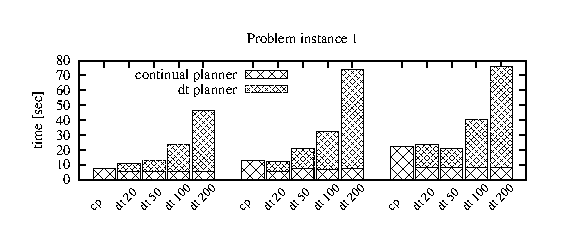
\includegraphics{dora1-time}\hfill
  % \vspace{2mm}
  \includegraphics{dora2-time}\hfill
  \vspace{2mm}
  \includegraphics{dora3-time}\hfill
  \vspace{2mm}
  \includegraphics{dora4-time}\hfill
  \vspace{2mm}
  \includegraphics{dora56-time}\hfill
  \vspace{2mm}
  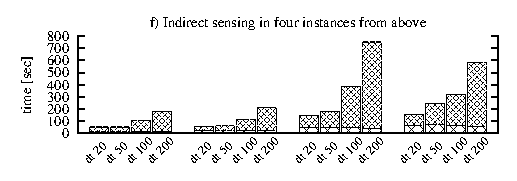
\includegraphics{dora-cat-time}\hfill
  \caption{Average runtime}
  \label{fig:results-time}
\end{figure}

\begin{figure}[h!]
  % \centering
  % \includegraphics{dora1-quality}\hfill
  % \vspace{2mm}
  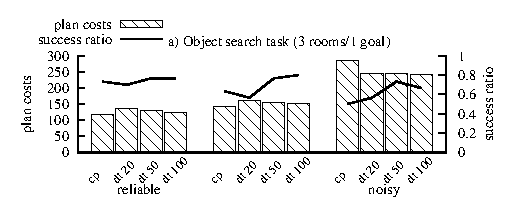
\includegraphics{dora2-quality}\hfill
  \vspace{2mm}
  \includegraphics{dora3-quality}\hfill
  \vspace{2mm}
  \includegraphics{dora4-quality}\hfill
  \vspace{2mm}
  \includegraphics{dora56-quality}\hfill
  \vspace{2mm}
  \includegraphics{dora-cat-quality}\hfill
  \caption{Average plan costs and number of successful runs}
  \label{fig:results-quality}
\end{figure}

The graphs in figure \ref{fig:results-time} show the average planning
times. Not surprisingly, the time the POMDP planner takes increases
strongly with larger belief spaces. But for the smaller belief states,
the cost for the decision theoretic planning is compensated by the
decrease of time spent in Fast Downward.

Figure \ref{fig:results-quality} shows the average costs of the
executed plans as well as the percentage of solvable tasks that were
actually solved by the planner. For objects that can be easily
detected there is little gain in using a decision theoretic planner,
as the greedy sensing appoach by the baseline continual planner is
obviously sufficient here. With decreasing sensor reliability the more
sophisticated observation planning pays off: while the resulting plans
are still longer on average, the impact on the number of solved tasks
was much smaller than for the baseline system.

As already mentioned, less aggressive pruning of the initial belief
space resultes in longer runtimes. The impace of the pruning on plan
costs and success rate were limited, though. Increasing the size limit
beyond 50 did rarely pay off because while additional information
might in theroy allow better plans, (add reason here). The indirect
sensing tests show the same result, though with much higher time spent
in the decision theoretic planner. The relatively high success rate
even with small belief spaces might also indicate that the entropy
heuristic for belief space pruning is effective in keeping the most
relevant information.

% We believe that a part of the improvement is due to the segmentation of
% the plan into several subtask, essentially performing hierarchical
% planning. Especially when the continual planner performs badly this is
% a huge gain.

%%% Local Variables: 
%%% mode: latex
%%% TeX-master: "moritz_2011"
%%% End: 


%% \section{Discussion}
%% 

A theoretical criticism of switching continual planning, concerns
interleaved sequential and decision-theoretic sessions failing to make
any progress towards the objective.


\section{Related Work}
There have been a number of developments recently moving towards
planning under uncertainty using systems that were intended for
sequential planning in deterministic problems.  Notably for example,
\system{FFR$_a$}~\cite{yoon:etal:2007}, the winning entry from the
probabilistic track of the 2004 International Planning Competition.
In the continual paradigm, \system{FFR$_a$} uses the fast satisficing
procedure \system{FF}~\cite{hoffmann:nebel:2001} to compute sequential
plans and corresponding execution traces.
%%
More computationally expensive approaches in this vein combine
sampling strategies on valuations over {\em runtime variables} with
deterministic planning procedures. The outcome is typically a more
robust sequential plan~\cite{yoon:etal:2008}, or contingent
plan~\cite{majercik:2006}. 

%%No! They simply haven't been evaluated in PO settings. They may, or
%%may not struggle. They have sampling of traces, and that would
%%include observations, and therefore evolutions of beliefs. SSAT was
%%proposed by Littman for POMDPs. So the majercik stuff is perfectly
%%suited to POMDPs.

% Normally if we are going to compare with related work, we do
% actually *compare*. Why didn't you try those approaches? I think
% it's safe to say that FFR will struggle. Why would it even include
% in its plan an observational action that doesn't change the world?

%%
%% However, as we said in the introduction,
%% all these approaches struggle in partially observable domains as they
%% rely on being able to determine the state at all times.

Also leveraging deterministic planners in problems that feature
uncertainty, \system{Conformant-FF}~\cite{hoffmann:brafman:2006} and
$T_0$~\cite{palacios:geffner:2009} demonstrate how conformant planning
---i.e., sequential planning in unobservable worlds--- can be modelled
as a deterministic problem, and therefore solved using sequential
systems. In this conformant setting, advances have been towards
compact representations of beliefs amenable to existing best-first
search planning procedures, and lazy evaluations of beliefs. Most
recently this research thread has been extended to contingent planning
in fully observable non-deterministic
environments~\cite{albore:etal:2009}.
%%
The continual planning system that motivated our
project~\cite{brenner:nebel:jaamas09} also has this characteristic,
and has been applied in completely observable domains, particularly
those featuring multiple communicating agents. The use of knowledge
operators in domains allows plans that act to gain knowledge, but the
approach assumes that such actions are deterministic and reliable, an
assumption that we relax in this work.

Our work is motivated by domains that contain a mixture of task
planning and observation planning. There have been a number of recent
papers representing observation planning problems as POMDPs and using
various techniques to manage the large state
space. \citeauthor{hippo-jnl}~(\citeyear{hippo-jnl}) take this
approach in a vision algorithm selection problem. In their case there
is a natural hierarchical decomposition of the problem which allows
them to solve large problems by breaking them into a set of small
POMDPs. \citeauthor{doshi08:pref_elic}~(\citeyear{doshi08:pref_elic})
represent a preference elicitation problem as a POMDP and take
advantage of symmetry in the belief space ---essentially the idea that
it does not matter what the value of the variable you are trying to
observe is--- to exponentially shrink the state space. Although we
have been actively exploring the \citeauthor{doshi08:pref_elic}
approach, we have yet to find those exploitable structures in our
domain due to the task planning requirement.


\section{Concluding Remarks}
\vspace{-1ex}

For use in an integrated continual planning and execution monitoring
system on a mobile robot platform, we developed a planner that
switches between: (a) fast sequential planning, and (b) expensive DT
planning in small abstractions of the problem at hand. Given a DTPDDL
model of the environment, sequential planning is used to compute an
initial sequential plan and complementary runtime evolution of the
decision process. That plan is executed until the outcome of the next
action scheduled for execution is too uncertain. At that point a DT
session performs sensing that can help determine how the sequential
plan might evolve, or otherwise acts to achieve the goals. We find our
approach performs quickly and relatively efficiently in a number of
large real-world task and observation planning problems.

\Omit{
The most pressing item for future research, is to develop a scheme
whereby the serial planner can relax {\em executability} assumptions,
so that conformant (or semi-conformant) plans can be executed without
interruption by a DT session. A more general criticism of
switching continual planning concerns interleaved sequential and
DT sessions failing to make any progress towards the
objectives. For example, in the worst case we can have each sequential
session producing an identical plan, and each decision-theoretic
session rejecting it without further sensing. Although this has not
been an issue in our work so far, it must be dealt with rigorously
in the future. We suggest that a good way to mitigate this problem is
by developing a {\em motivational} component that maintains a {\em
dynamic} reward model whose limiting behaviour prevents that switching
deadlock.
}




%% The sequential mode of our system always schedules decision-theoretic
%% planning before executing actions that are not applicable with
%% certainty. This is inefficient if the utility of the plan is not
%% dependent on that actions successful execution. This situation always
%% arises for conformant plans. 



%% The switching continual planning system we have described serves as
%% the underlying planner for CogX.




%% the effects of a {\em sense} schema are perceptual, whereas the
%% effects of an {\em operator} schema are over state propositions.




%% posted by a motivational component of the underlying robotic
%% architecture. 

%% contingent sensory plans that are tailored to current
%% objectives.

%% In this paper we present an approach to continual planning that uses
%% two planning systems. The first 
				   
%%  to a distinct class of
%% challenges. We suppose 
%% %%
%% The underlying environment is modelled as a POMDP. We use the fast
%% classical satisficing system FastDownward to find a deterministic
%% sequential plan and complementary runtime evolution of that
%% process. This corresponds to a generalisation of replanning in
%% probabilistic planning to problems with partial observability.

%% Interaction between the sequential planner and execution proceeds
%% more-or-less analogously to popular replanning approaches

%% Addressing these challenges in a monolithic framework, we present a
%% {\em switching} continual planner, that uses the fast sequential
%% satisficing procedure FastDownward to perform net-benefit
%% %%
%% makes reasonable assumptions about the evolution of the runtime state
%% given a POMDP model of the environment. 

%% contingent sensory plans that are tailored to current
%% objectives.


%% The decision-theoretic planner is able to tailor sensory processing on
%% a robot platform to the current objective, while FastDownward  quickly 


%% In this paper we develop a continual planing system that uses two
%% planning systems. The first, is a state-of-the-art domain independent
%% planner for deterministic problems. The second is a information-state
%% contingency planning the information-state space of 


%% Continual planning is a powerful technique that goes some way to
%% addressing those challenges. That approach interleaves planning and
%% execution, deliberately postponing planning for contingencies unless
%% they eventuate during execution. 


%% computing a single sequential plan and
%% eventuality



%% To these challenges it seems a continual planning approach is best, 

%% where the runtime state evolves during plan execution 


%% interleaved planning and execution. 

%% the latter is able to tailor sensory processing on a robot platform,
%% in order that it.

%% {\em ad-hoc} 

%% , reason about degrees of belief and uncertainty about the world, 

%% probabilistic sequential decision making in practical sized problems
%% is intractable.

%% quantitative probabilistic models of the perception and action .



\bibliographystyle{aaai}
\bibliography{papers}

\end{document}


























\subsection{PPDDL}

We briefly discuss the description language PPDDL, a fairly
straight-forward extension of the Planning Domain Definition Language
for describing fully observable Markov decision processes.

\small{
\begin{tabtt}
(\= :action look-at-object \\
  \> :parameters \=(?r - robot ?v - visual-object\\
  \> \> ?l - label ?l - location) \\
  \> :precondition (and (= (is-in ?r) ?l) \\
  \> \> (= (label ?o) ?l) ) \\
  \> :effect (and (assign (reward) -3) ) ) \\
\end{tabtt}
}

\small{
\begin{tabtt}
(\= :observe visual-object \\
  \> :parameters \=(?r - robot ?v - visual-object\\
  \> \> ?l - label ?l - location) \\
  \> :execution (look-at-object ?r ?v ?l ?l) \\
  \> :effect (when (= (is-in ?o) ?l) (probabilistic 0.8)) \\
\end{tabtt}
}

\small{
\begin{tabtt}
(\= :sensor look-for-object \\
  \> :agent (?a - robot) \\
  \> :parameters (?l - label ?l - location) \\
  \> :variables (?o - visual-object) \\
  \> :precondition (\=and (= (is-in ?r) ?l) \\
  \> \> (= (label ?o) ?l) (assume (is-in ?o) ?l) ) \\
  \> :effect () \\
  \> :sense (= (is-in ?o) ?l) \\
\end{tabtt}
}

\subsection{MAPL}



%% \scriptsize
%% \begin{nopagebreak}\begin{tabtt}
%% <observation-def> \=::= \=(:sense <observation symbol> \\
%%                         \> \> :parameters (<typed list (variable)>)  \\
%%                         \> \> <o-def body>) \\
%%   <o-symbol> \> ::= <name> \\
%%   <o-def body> \> ::= [:precondition <GD>] \\
%%   \> \> [:execution <atomic action(term)> ] \\
%%     \> \> [:effect <o-effect>] \\
%%   <atomic action(t)> \> ::= (<action symbol> t\zom) \\
%%   <o-effect> \> ::= (and <c-o-effect>\zom) \\
%%   <o-effect> \> ::= <c-o-effect> \\
%%   <c-o-effect> \> ::= \req{:probabilistic-effects} (probabilistic <prob> <o-effect>) \\
%%   <c-o-effect> \> ::= <p-o-effect> \\
%%   <atomic o-formula(t)> \> ::= (<observation> t\zom) \\
%%   <p-o-effect> \> ::= <atomic o-formula(term)> \\
%%   <p-o-effect> \> ::= (not <atomic o-formula(term)>) \\
%%   <o-f-comp> \> ::= (<binary-comp> <o-f-exp> <o-f-exp>)\\
%%   <o-f-exp> \> ::= <number>\\
%%   <o-f-exp> \> ::= (- <o-f-exp>)\\
%%   <o-f-exp> \> ::= <o-f-head>\\
%%   <o-f-head> \> ::= (<o-function-symbol> <term>\zom )\\
%%   <o-f-head> \> ::= <o-function-symbol>\\
%% \end{tabtt}\end{nopagebreak}
%% \noteme{<structure-def> ::= <attach-def>}
%% \normalsize



%% \footnote{We have simplified the schemata for illustrative
%% purposes. In practice, the probabilities of a particular observation
%% here should be parametrised by the type of visual object the robot is
%% searching for, and category of the location.}


We suppose $\bstate_0$ is given in a factored tree format of the
form:


%% \small{
%% \begin{tabtt}
%% (:init  (and \=f_{11} f_{12} ..
%%  \> (probabilistic p_{}) 
%%  \> (probabilistic ..) ..) \\
%% \end{tabtt}
%% }

%% \[(:\pp{init} (and f_{11} f_{12} .. (\pp{probabilistic} p_) ))\]


planning in practical sized POMDPs is intractable. One approach is to
described the task hierarchically, thereby constrain and simplify the
policy search task. The approach ~\cite{}. 


%% More generally, a useful
%% formalism for representing solutions to POMDPs is the finite-state
%% controller (FSC). This is a three-tuple $\langle \nodes, \selection,
%% \transition \rangle$ where: $\node \in \nodes$ is a set of nodes,
%% $\selection_\node(\action) = P(\action | \node)$, and
%% $\transition_\node(\action, \observation, \node') = P(\node'|\node,
%% \action, \observation)$. Where the value of acting is the discounted
%% accumulated reward over an infinite horizon, then each controller can
%% be assigned a value, written $V_\node(\state)$, expressed in the usual
%% way according to the Bellman equation:

%% \begin{equation}\label{eq:evaluation}
%% \begin{array}{lcl}
%% V_\node(\state) & = & \sum_{\action \in \actions}
%% \selection_\node(\action) \reward(\state, \action) \;\; + \vspace{1ex} \\

%% && \hspace{-10ex} \beta \sum_{\action, \observation,
%% \state', \node'} \transition_\node(\action, \observation, \node')
%% \transProb(\state, \action, \state') \obsDist_\observ(\state',
%% \action) V_{\node'}(\state')
%% \end{array}
%% \end{equation}

%% \noindent Here, the value of {\em prior} $\bstate$ given an FSC is
%% then:

%% \begin{equation} \label{eq:valueBelief}
%% V_{\pp{FSC}}(\bstate) = \max_{\node \in \nodes} \sum_{\state \in \states} \bstate(\state) V_\node(\state)
%% \end{equation}

%% \noindent There is a corresponding deterministic FSCs for both
%% sequential (i.e., conformant) and contingent
%% plans. Eq~\ref{eq:evaluation} gives their value in the finite-horizon
%% case, if we take $\beta = 1$, and alter the process dynamics so there
%% is a compulsory transition to a zero utility sink state when that
%% horizon is reached.


 ---i.e., the values of {\em
runtime variables} in the continual paradigm--- are treated , and
therefore plan for a specific eventuality, replanning from scratch if
something




Sequential planning in our approach proceeds in two phases. In the
first phase, the goal is to identify a plan prefix

In sequential planning, the plan prefix corresponds to choosing a
valid abstract starting state. 

moreover, for the purpose of decision-theoretic abstractions, 


A relaxed form of {\em visitation} we call {\em abstract
  visitation}. In the abstract case a conjunctive term is visited
  provided all its atomic subterms are visited, and zero or more of
  its probabilistic terms are visited.

The planner has a compulsory starting action, that visits the root
term, and then has to execute visitation actions until that plan
prefix corresponds to a valid {\em abstract visitation} of the {\em
:init} decleration. Beyond such a prefix, the process actions and senses are
available to the planner 


Goal expressions in the problem description ---for example
$(\pp{kval}~(\pp{location}~\pp{box}))$ expresses ``the robot knows the
location of the {\em box}--- are treated as control-knowledge by the
planner. Here, a plan is not considered valid unless in the finial
stet the goal condition is satisfied.
